\section{ggplot2 part 4}
\begin{frame}\frametitle{themes}
  \begin{itemize}
  \item themes can be used to customize the visual appearance of the plot
  \item theme elements can inherit properties from other theme elements
  \item the modification is done element by element inside \texttt{theme()}
  \item there are some themes included in the ggplot2 package and there are more in ggthemes or on the web
  \end{itemize}
\end{frame}


\begin{frame}\frametitle{Text styles}
  \begin{itemize}
  \item the element to modify is an \texttt{element\_text()}
  \item typical elements are:
    \begin{itemize}
    \item \texttt{title} 
    \item \texttt{axis.title.x/y} inherits from \texttt{axis.title} inherits from \texttt{title}
    \item \texttt{axis.text.x/y} inherits from \texttt{axis.text}
    \item \texttt{legend.text} and \texttt{legend.title}
    \item \texttt{axis.strip.x/y} inherits from \texttt{strip.text}
    \end{itemize}
  \end{itemize}
\end{frame}


\begin{frame}[allowframebreaks]\frametitle{element\_text() options}
  \begin{itemize}
    \item \texttt{family}: font family
    \item \texttt{face}: font face (plain, italic, bold, bold.italic)
    \item colour: text colour
    \item size: text size (in pts)
    \item hjust: horizontal justification (in [0, 1])
    \item vjust: vertical justification (in [0, 1])
    \item angle: angle (in [0, 360])
    \item lineheight: line height
    \item color: an alias for ‘colour’ 
  \end{itemize}
\end{frame}

\begin{frame}[fragile,allowframebreaks]\frametitle{Example Data}
\scriptsize
\begin{verbatim}
> p1 <- ggplot(dl,aes(x=variable,y=value,colour=group)) +
+     geom_boxplot(aes(x=variable,group=factor(variable))) +
+     stat_summary(fun.y="mean",geom = "line") +
+     ggtitle("Plot title")
> p1 + theme(
+     title = element_text(colour="red", face="bold", angle = 10),
+     axis.title.y = element_text(colour="blue", face="italic",size=25)
+ )
\end{verbatim}
  \begin{center}
    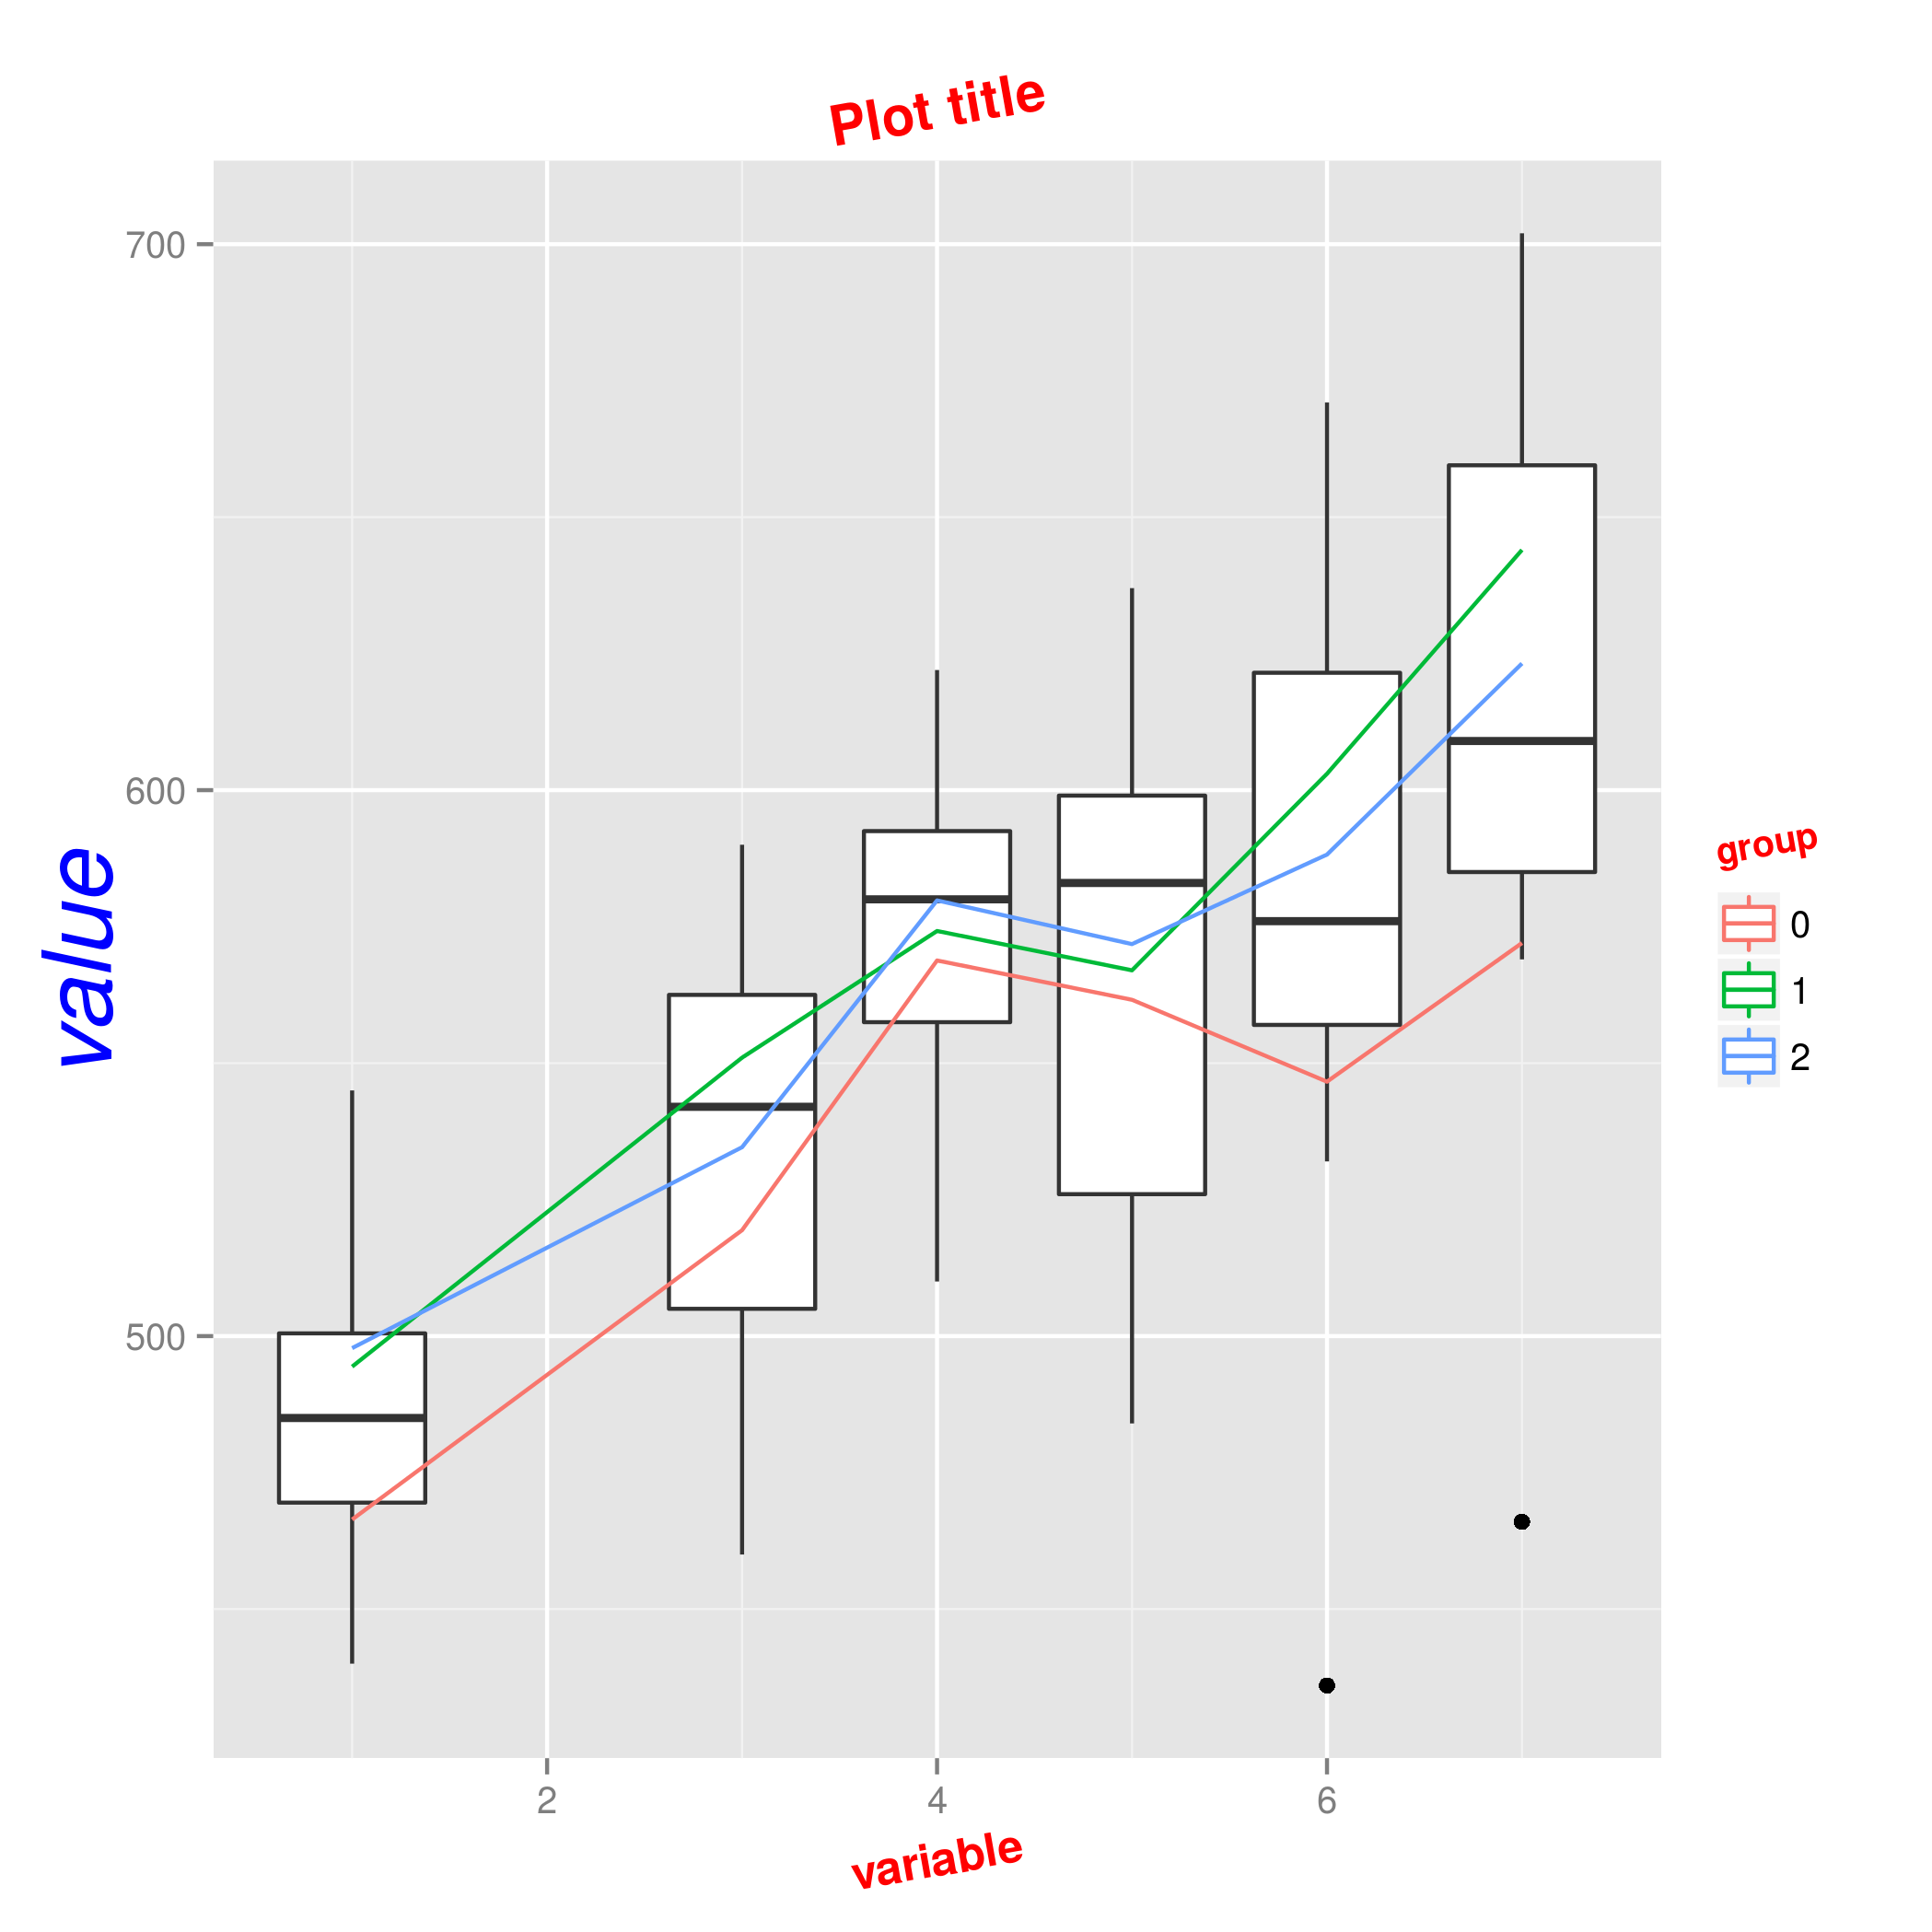
\includegraphics[width=11cm, height=7cm]{ggtext.png}
  \end{center}
\end{frame}



\begin{frame}\frametitle{Line styles}
  \begin{itemize}
  \item the element to modify is an \texttt{element\_line(elem)}
  \item typical elements are:
    \begin{itemize}
    \item \texttt{axis.line.x/y} inherits from \texttt{axis.line}
    \item \texttt{axis.ticks.x/y} inherits from \texttt{text.text}
    \item \texttt{panel.grid.minor/major.x/y} and \texttt{panel.grid}
    \end{itemize}
  \end{itemize}
\end{frame}

\begin{frame}\frametitle{element\_line() options}
  \begin{itemize}
  \item colour: line colour
  \item size: line size
  \item linetype: line type
  \item lineend: line end
  \item color: an alias for ‘colour’ 
  \end{itemize}
\end{frame}


\begin{frame}[fragile,allowframebreaks]\frametitle{Example Data}
\scriptsize
\begin{verbatim}
> p1 + theme(
+     axis.line = element_line(colour="green", linetype = 3, size = 3)
+ )
\end{verbatim}
  \begin{center}
    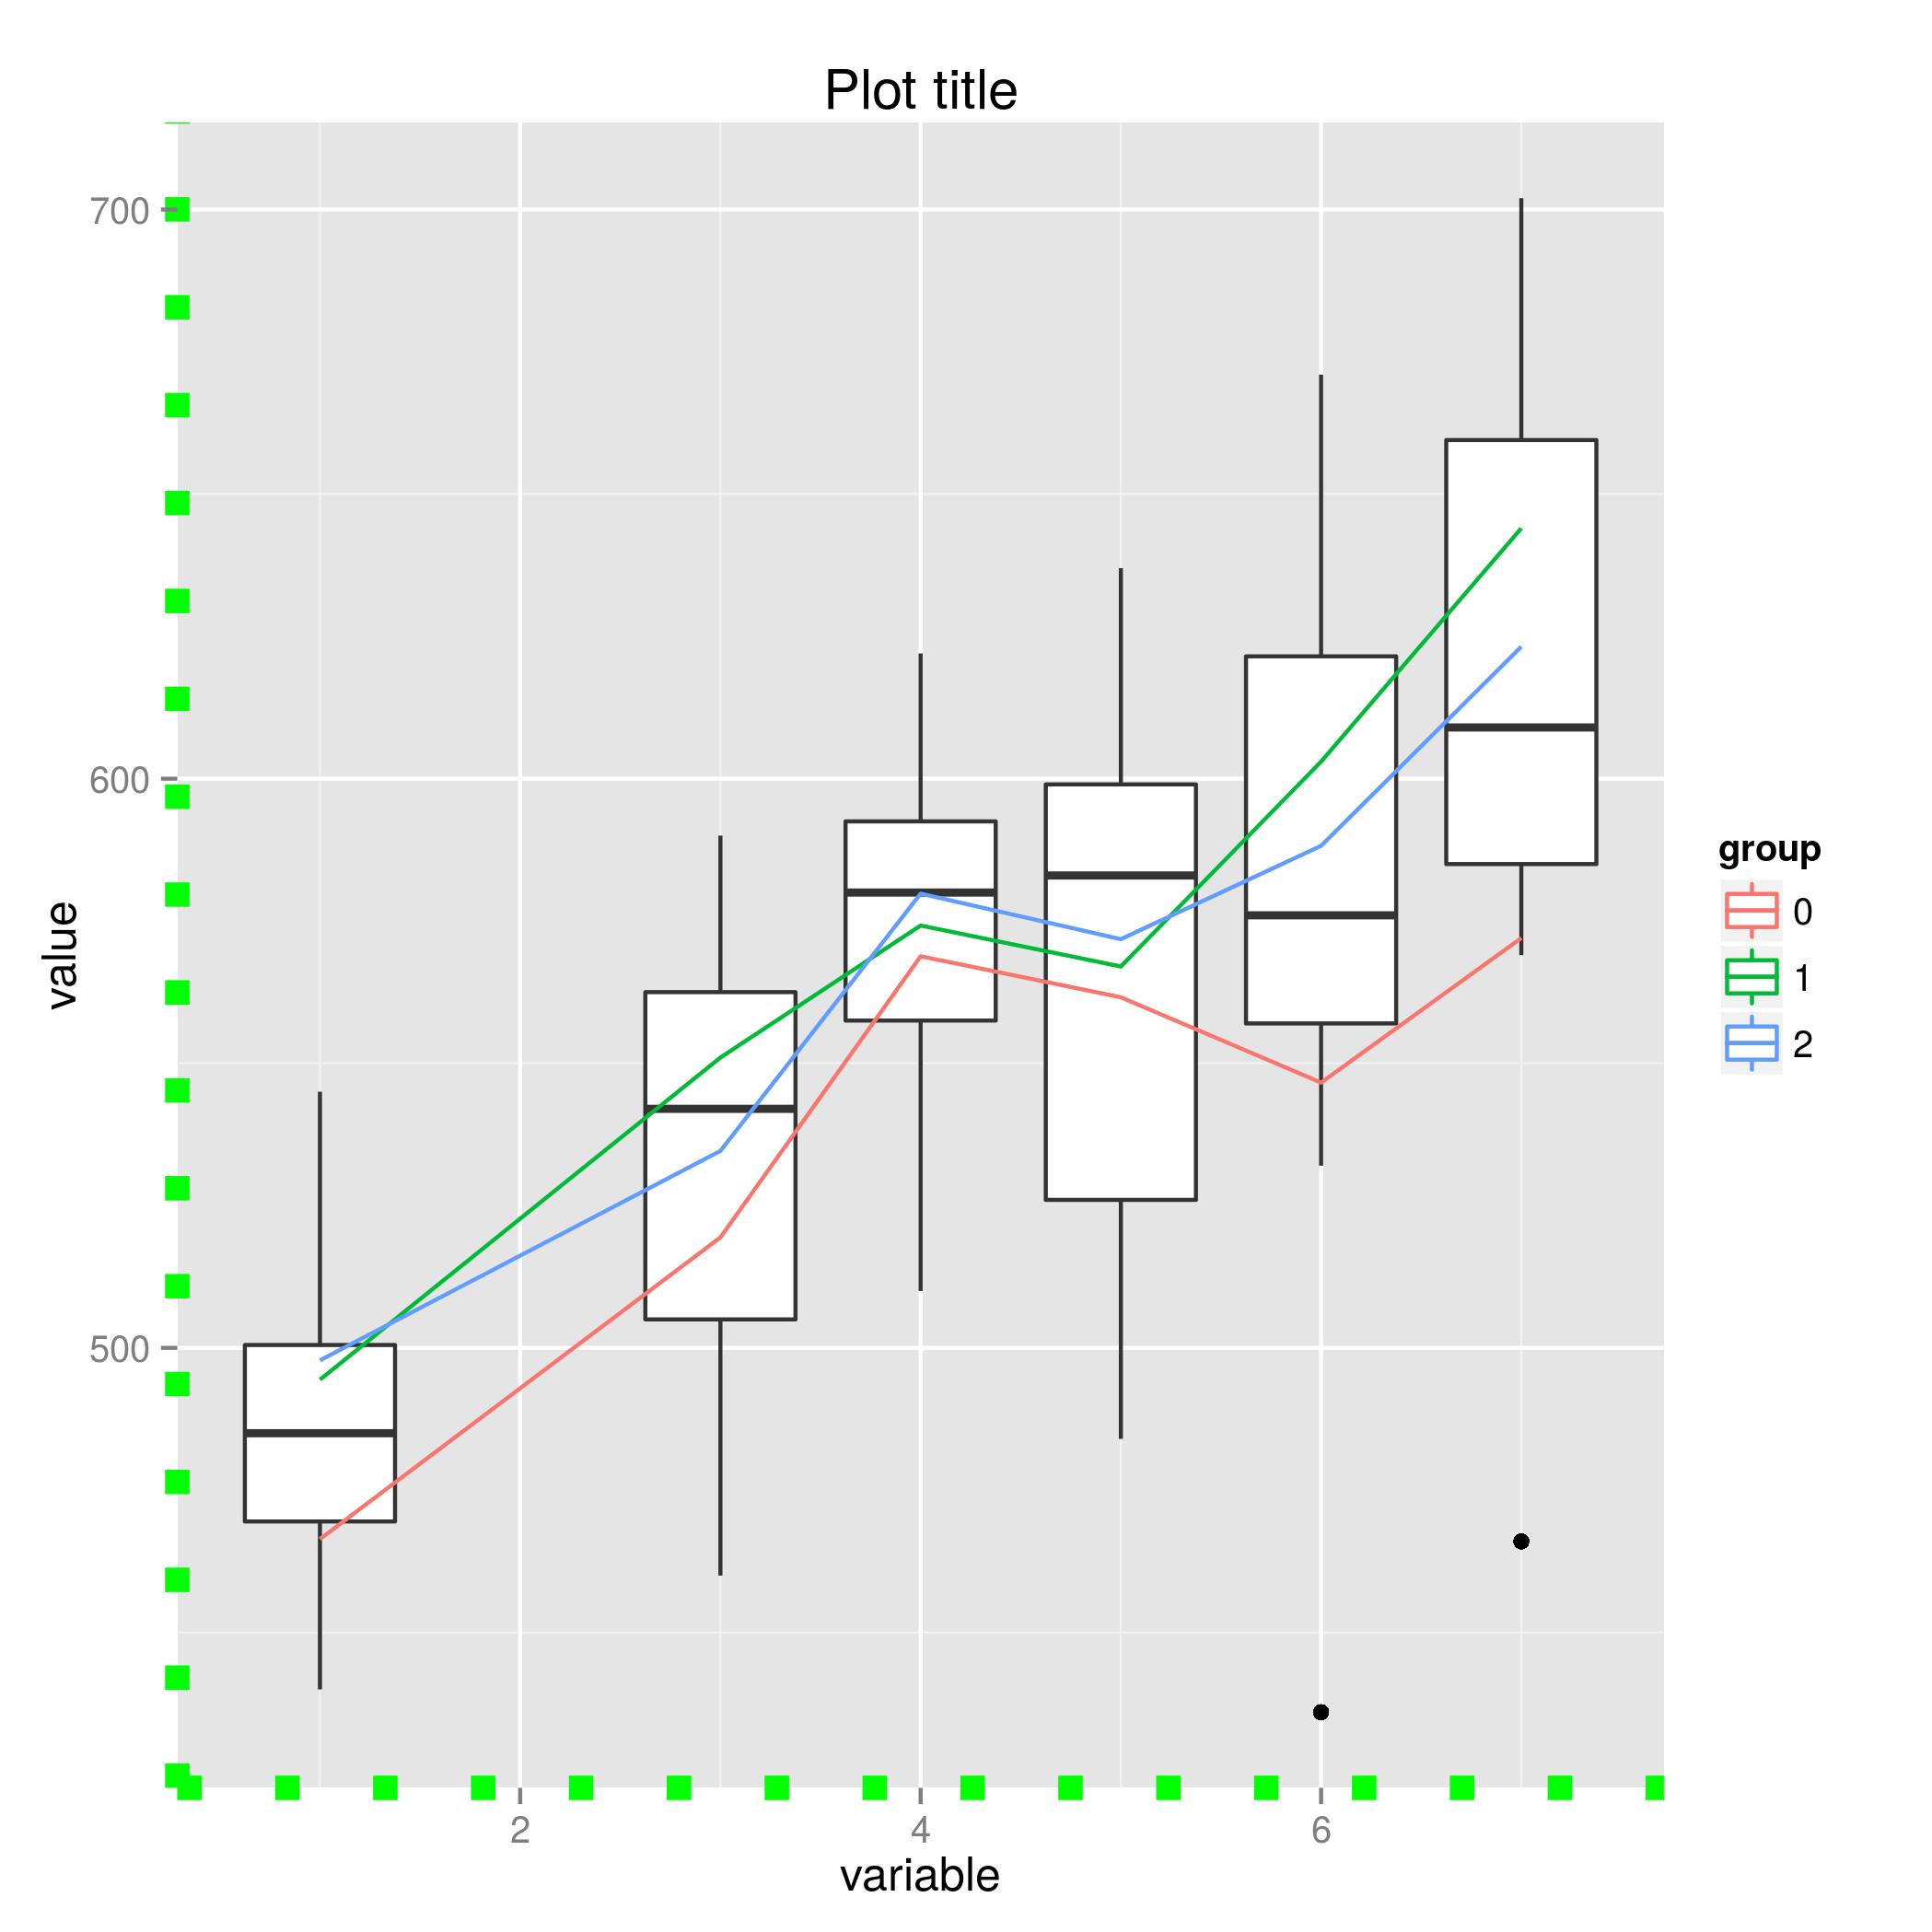
\includegraphics[width=11cm, height=7cm]{ggline.png}
  \end{center}
\end{frame}

\begin{frame}[fragile,allowframebreaks]\frametitle{Example Data}
\scriptsize
\begin{verbatim}
> p1 + theme(
+     axis.line = element_line(colour="green", linetype = 3, size = 3),
+     axis.ticks = element_line(colour="red", linetype = 3, size = 3),
+     panel.grid.major = element_line(colour="deeppink", linetype = 2, size = 1)
+ )
\end{verbatim}
  \begin{center}
    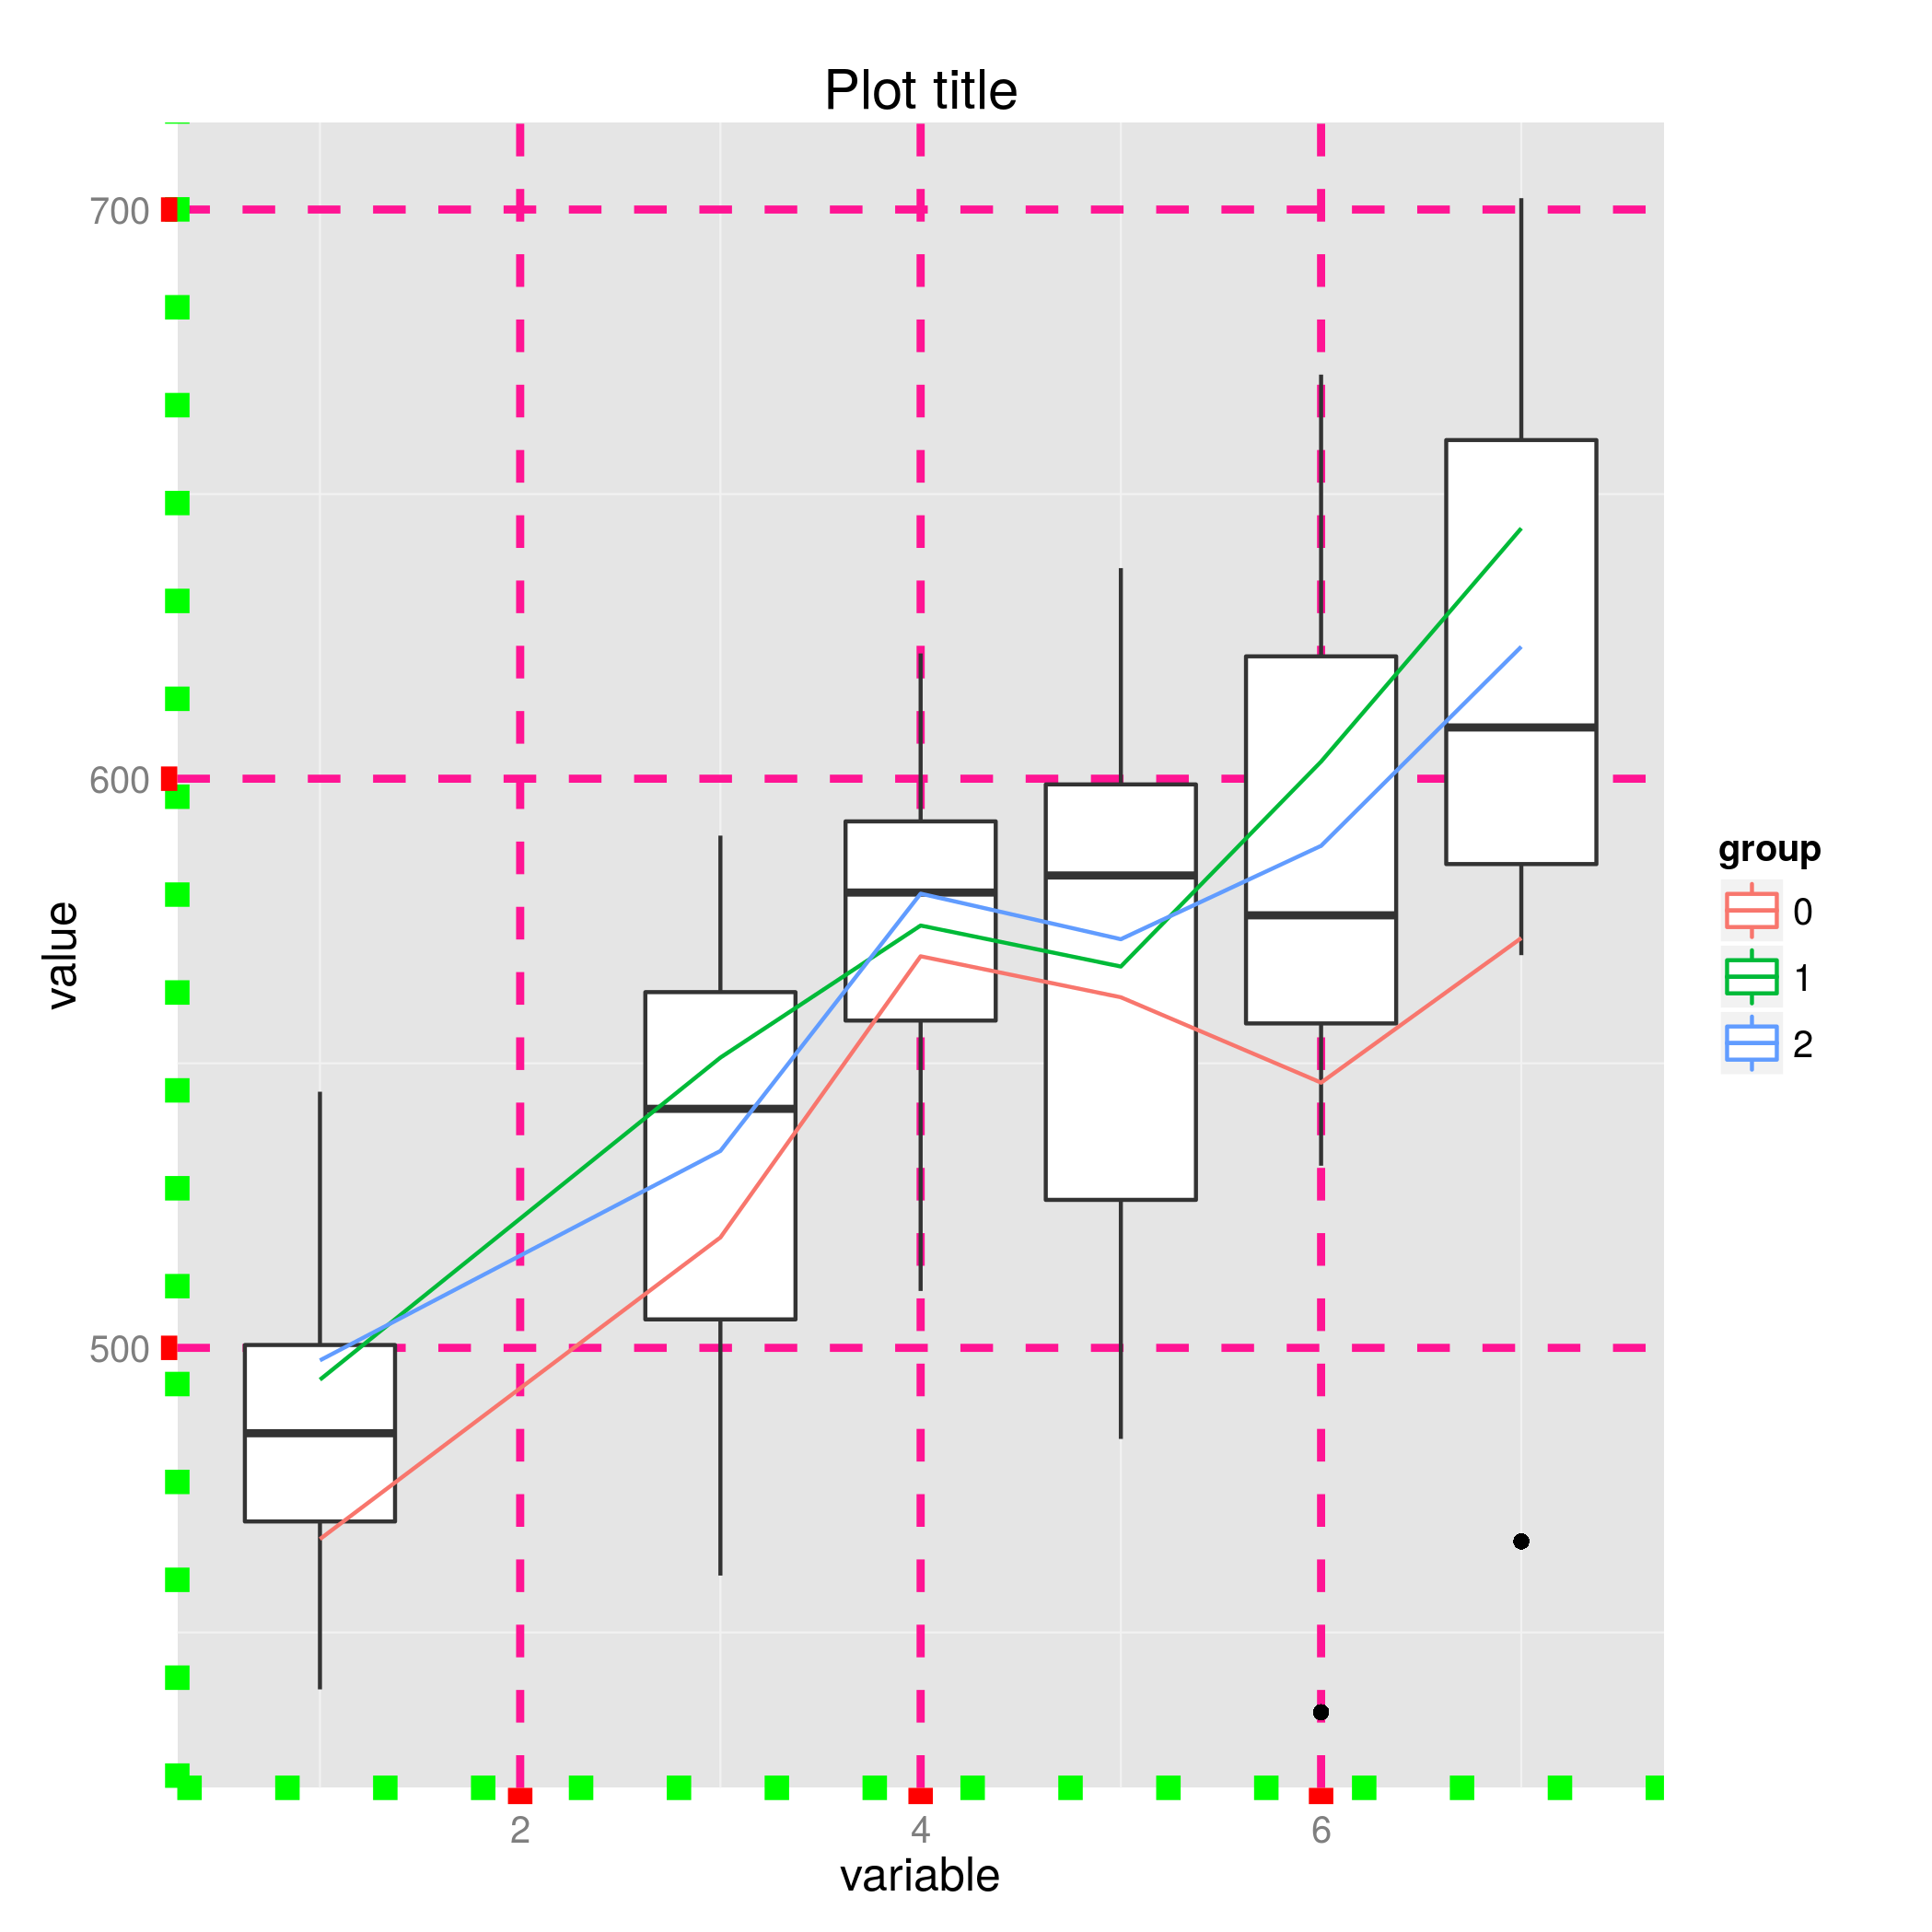
\includegraphics[width=11cm, height=7cm]{ggline2.png}
  \end{center}
\end{frame}



\begin{frame}\frametitle{Rectangular styles}
  \begin{itemize}
  \item the element to modify is an \texttt{element\_rect(elem)}
  \item typical elements are:
    \begin{itemize}
    \item \texttt{legend.background}
    \item \texttt{legend.key} 
    \item \texttt{panel.background}
    \item \texttt{plot.background}
    \item \texttt{strip.background}
    \end{itemize}
  \end{itemize}
\end{frame}

\begin{frame}\frametitle{element\_rect() options}
  \begin{itemize}
  \item fill: fill colour
  \item colour: border colour
  \item size: borer size
  \item linetype: border linetype
  \item color: an alias for ‘colour’ 
  \end{itemize}
\end{frame}


\begin{frame}[fragile,allowframebreaks]\frametitle{Example Data}
\scriptsize
\begin{verbatim}
> p1 + theme(
+     legend.background = element_rect(fill = "darkslategray1"),
+     panel.background = element_rect(fill = "darkslategray3"),
+     plot.background =  element_rect(fill = "darkslateblue")
+ )
\end{verbatim}
  \begin{center}
    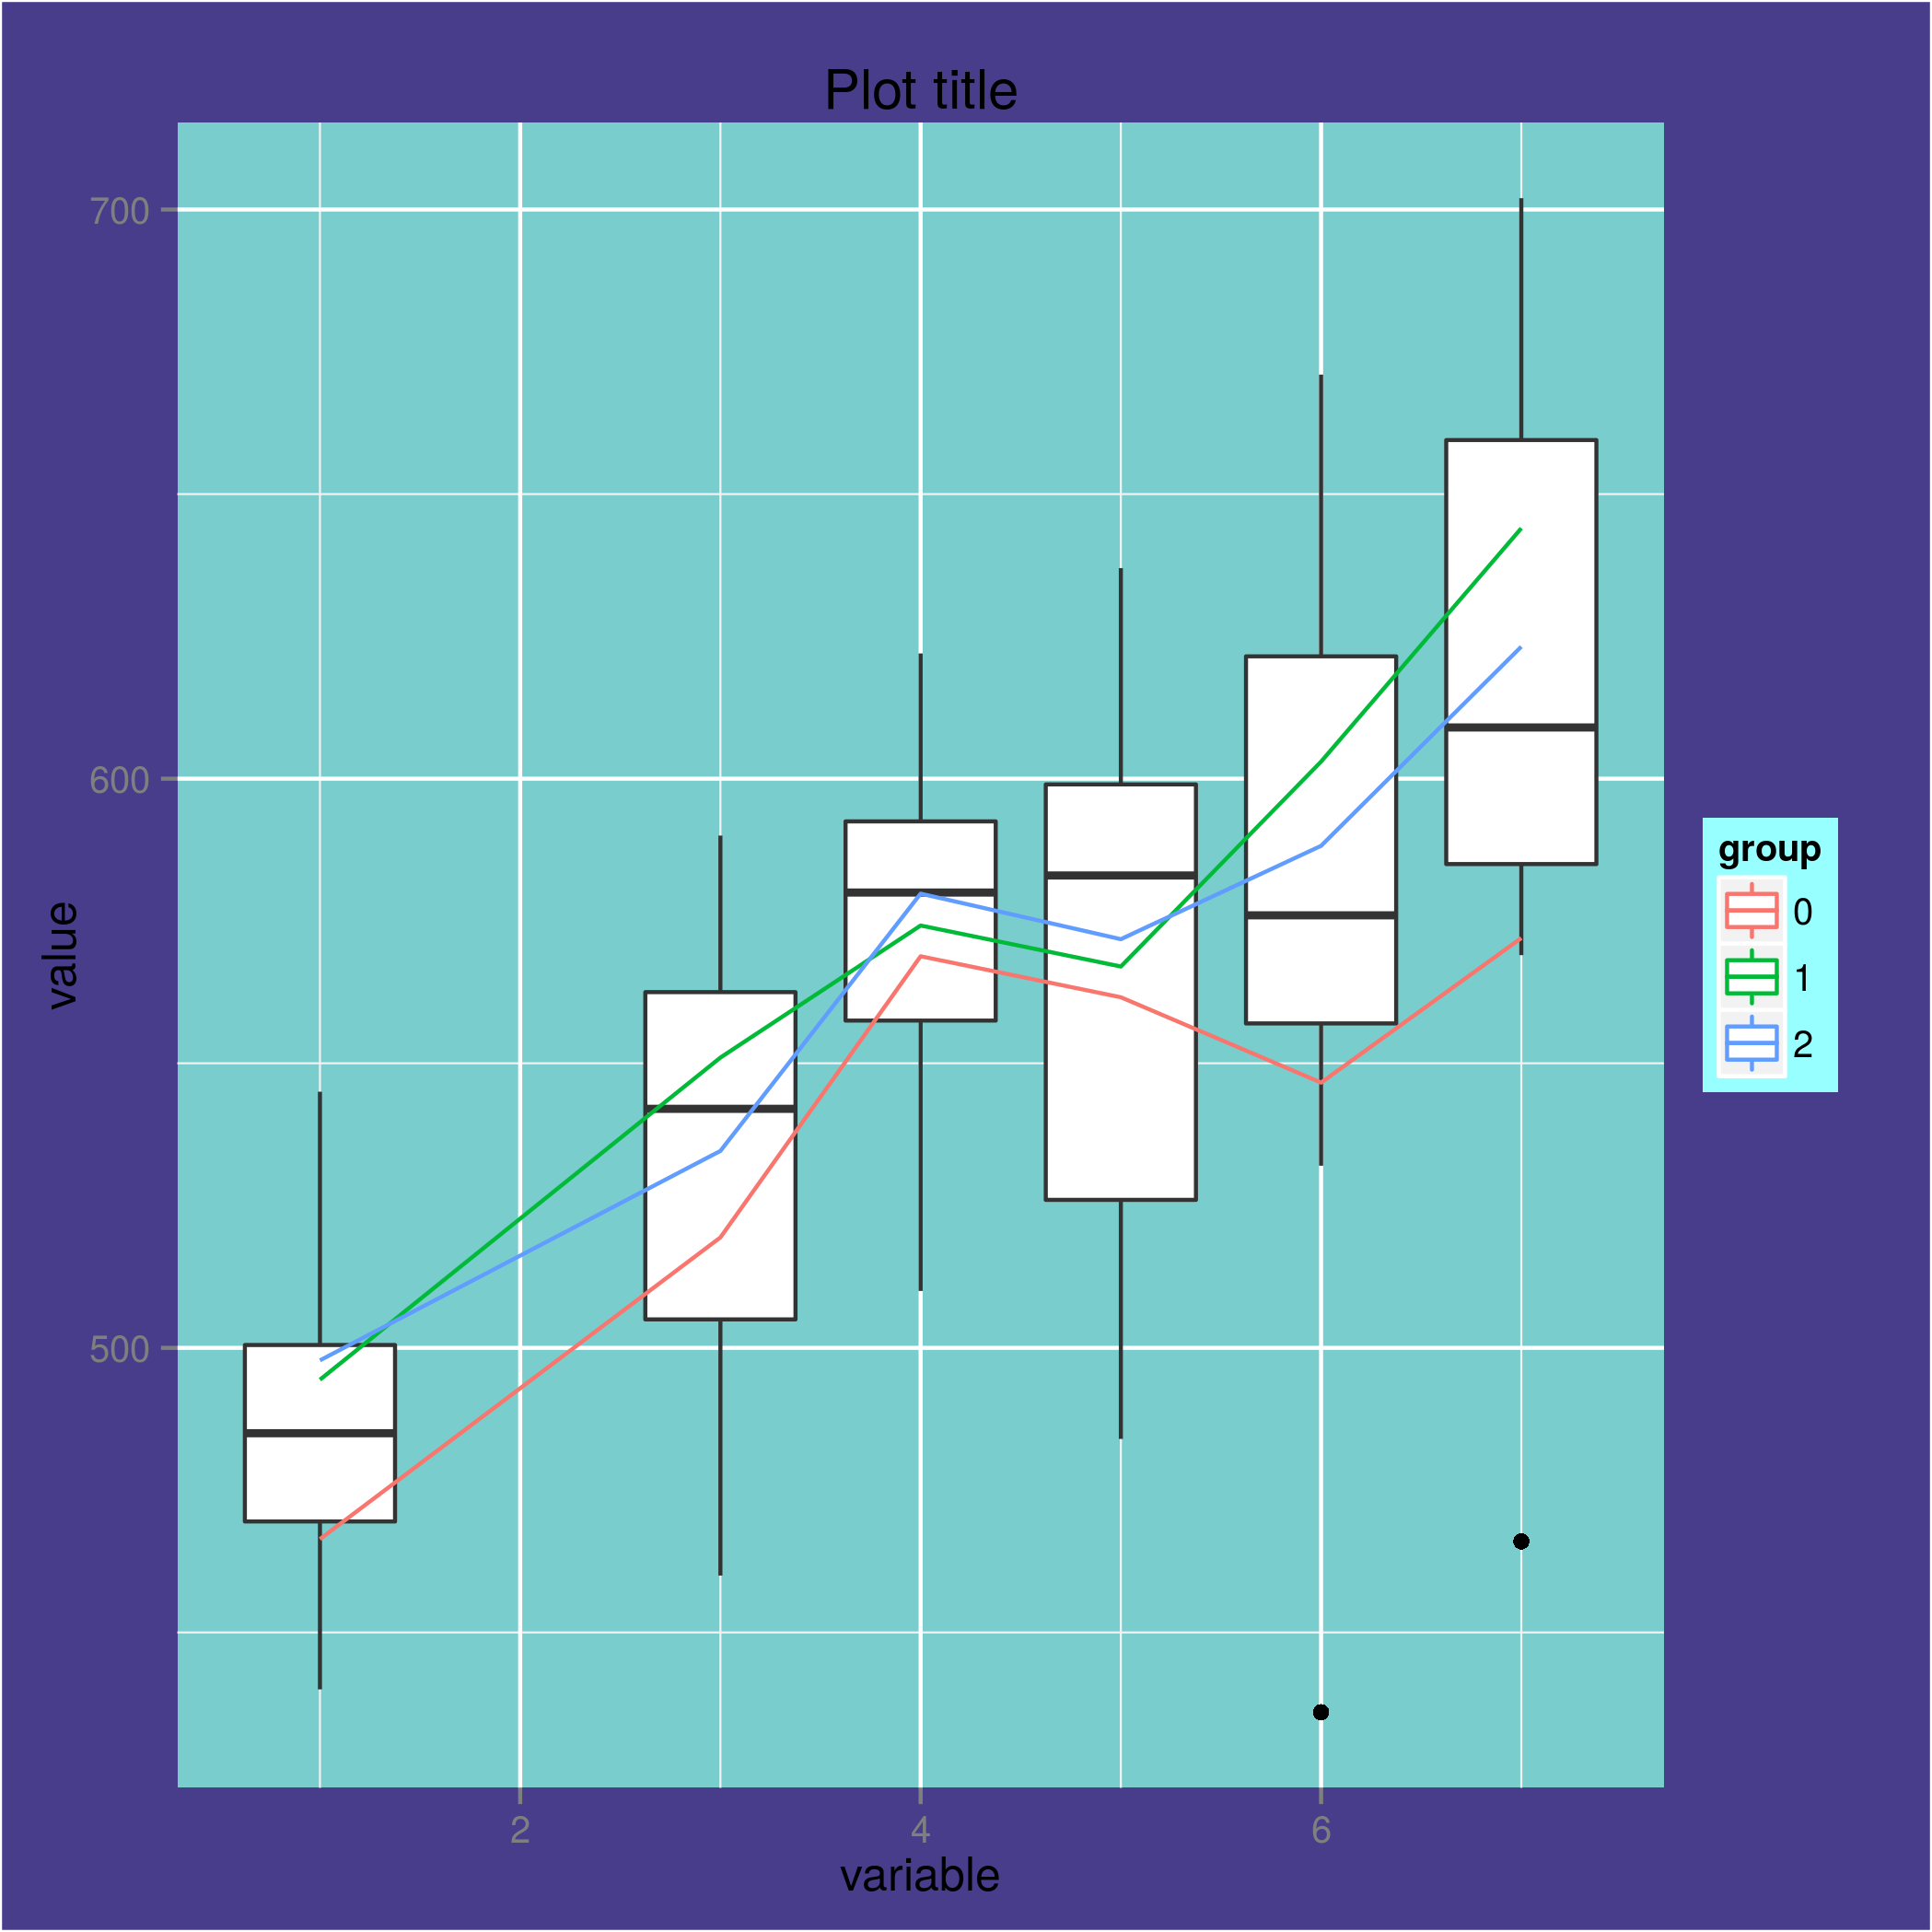
\includegraphics[width=11cm, height=7cm]{ggrect.png}
  \end{center}
\end{frame}



\begin{frame}[allowframebreaks]\frametitle{other options}
  \begin{itemize}
  \item legend.title.align 
  \item legend.position (none,left,right,bottom,top or relative position)
  \item legend.direction (horizontal or vertical)
  \item legend.justification
  \item legend.box (horizontal or vertical - arrangment of multiple legends)
  \item legend.box.just
  \item legend.key.size (unit)
  \item legend.key.height (unit)
  \item legend.key.width (unit)
  \item axis.ticks.length (unit)
  \item axis.ticks.margin (unit)
  \item plot.margin (unit) - margin around the plot
  \item etc
  \end{itemize}
\end{frame}


\begin{frame}[fragile, allowframebreaks]\frametitle{Example Data}
\scriptsize
\begin{verbatim}
> p1 + theme(
+     axis.ticks = element_line(colour="red", linetype = 2, size = 1),
+     axis.ticks.length = unit(1,"cm"),
+     axis.ticks.margin = unit(1,"cm"),
+     legend.position = c(0.5,0.5),
+     legend.background = element_rect(fill="transparent"),
+     legend.key.size = unit(2,"cm")
+ )
\end{verbatim}
  \begin{center}
    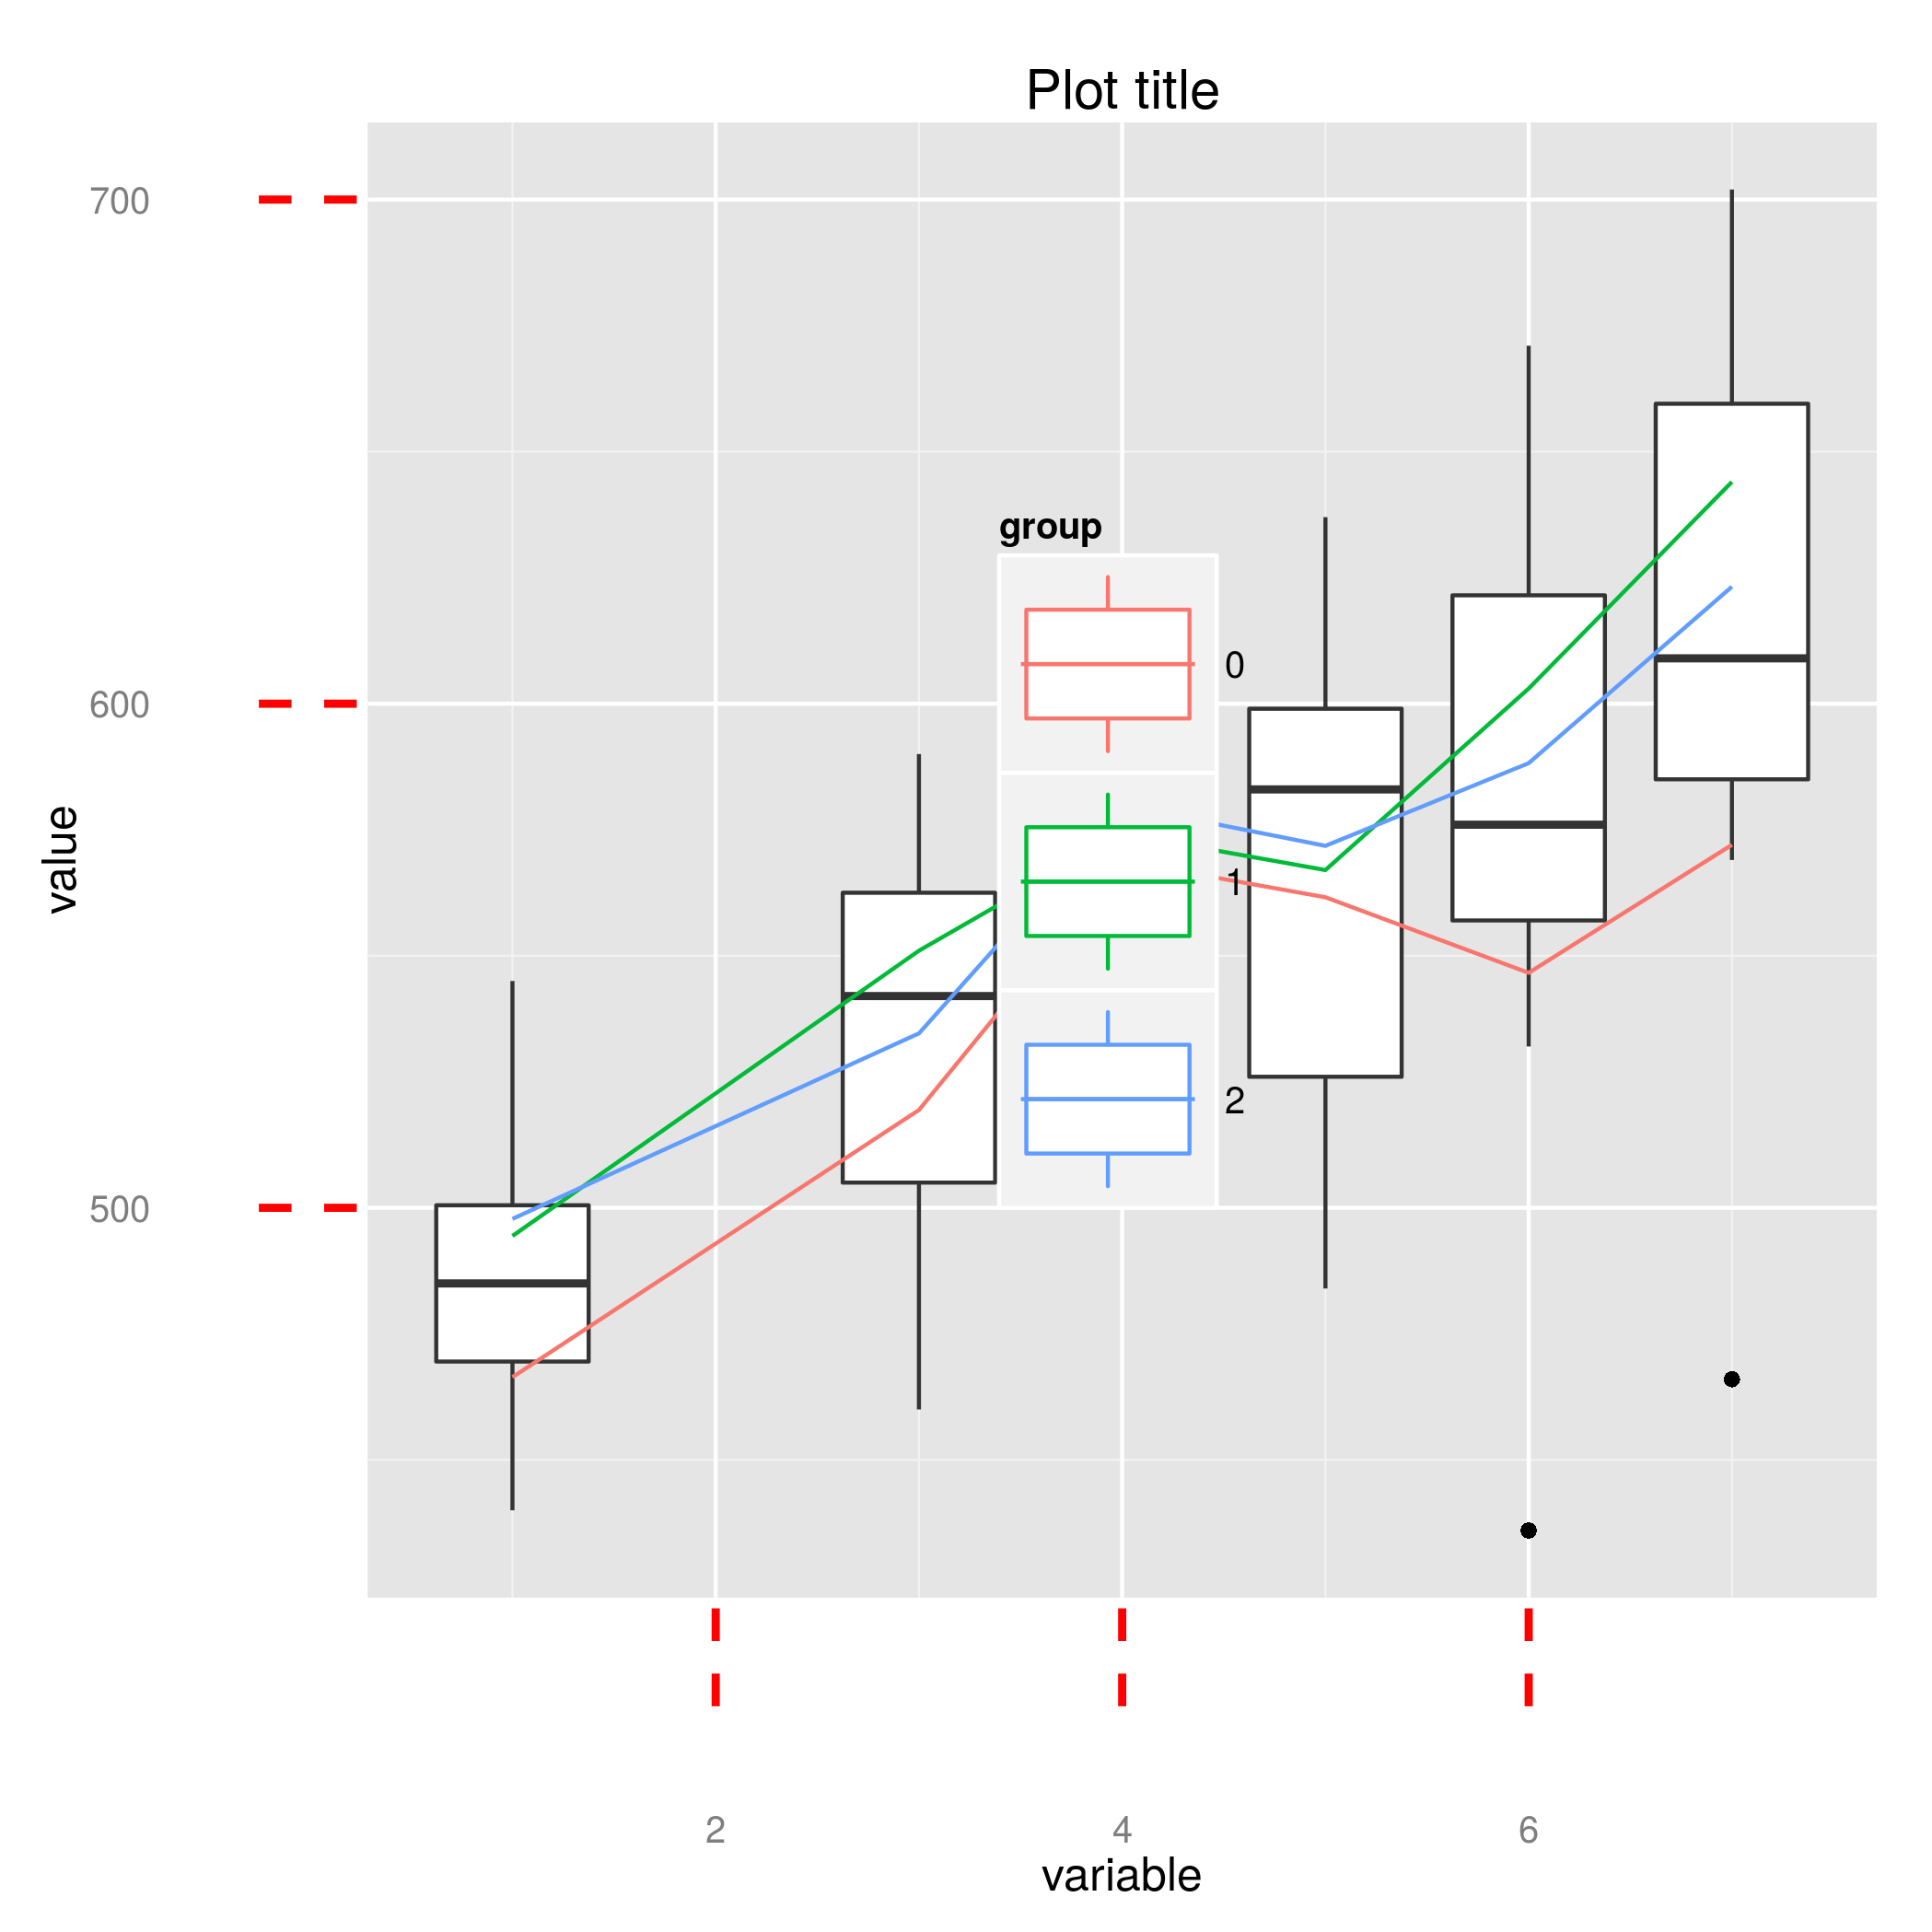
\includegraphics[width=11cm, height=7cm]{ggother.png}
  \end{center}
\end{frame}

\begin{frame}[fragile]\frametitle{Exercises}
  \begin{enumerate}
  \item download the data from the nih:\tiny
\begin{verbatim}
brfss <- read.csv("http://watson.nci.nih.gov/~sdavis/tutorials/IntroToR/BRFSS-subset.csv")  
\end{verbatim}
\normalsize
  \item use dplyr to create a new data frame summarising Age, Height, Weight per Year and Sex, calculate means, min, max, medians, number of observations, number of missing ages
  \item calculate BMI in the brfss data set make an appropriate plot to compare Weight, Height and Age of the sample per Year and sex. Hint: maybe you want transform the data before plotting using melt() from the reshape2 packageadd time as fixed effect.
  \item customize the plot, try to remove all elemets except the boxplot and the text elements
  \item change the colour scale (if you used one)
  \end{enumerate}
\end{frame}


\begin{frame}[fragile,allowframebreaks]\frametitle{Exercises - Solutions}
  \begin{enumerate}
  \item download the data from the nih:\scriptsize
\begin{verbatim}
brfss <- read.csv("http://watson.nci.nih.gov/~sdavis/tutorials/IntroToR/BRFSS-subset.csv")  
\end{verbatim}
\normalsize
  \item use dplyr to create a new data frame summarising Age, Height, Weight per Year and Sex, calculate means, min, max, medians, number of observations, number of missing ages\scriptsize
\begin{verbatim}
> require(dplyr)
> brfss %>% group_by(Sex,Year) %>%
+     summarise(mean.age = mean(Age,na.rm = T),
+               median.age = median(Age,na.rm = T),
+               min.age = min(Age,na.rm = T),
+               max.age = max(Age,na.rm = T),
+               mean.height = mean(Height,na.rm = T),
+               median.height = median(Height,na.rm = T),
+               min.height = min(Height,na.rm = T),
+               max.height = max(Height,na.rm = T),
+               mean.weight = mean(Weight,na.rm = T),
+               median.weight = median(Weight,na.rm = T),
+               min.weight = min(Weight,na.rm = T),
+               max.weight = max(Weight,na.rm = T),
+               nobs = n(),
+               n.missing = sum(is.na(Age)))
Source: local data frame [4 x 16]
Groups: Sex

     Sex Year mean.age median.age min.age max.age mean.height median.height
1 Female 1990 46.23327         42      18      99    163.3367        162.56
2 Female 2010 57.08824         58      18      99    163.2524        163.00
3   Male 1990 43.90552         41      18      94    178.2010        177.80
4   Male 2010 56.24993         57      18      99    178.0066        178.00
Variables not shown: min.height (dbl), max.height (dbl), mean.weight (dbl),
  median.weight (dbl), min.weight (dbl), max.weight (dbl), nobs (int),
  n.missing (int)
\end{verbatim}
\normalsize
  \item calculate BMI in the brfss data set make an appropriate plot to compare Weight, Height and Age of the sample per Year and sex. Hint: maybe you want transform the data before plotting using melt() from the reshape2 packageadd time as fixed effect.
\scriptsize
\begin{verbatim}
> brfss$bmi <- brfss$Weight/(brfss$Height**2) * 10000
> 
> dl <- melt(brfss,id.vars = c("Sex","Year"))
> ggplot(dl,aes(x=factor(Year),y=value,fill=Sex)) +
+     geom_boxplot() +
+     facet_wrap(~variable,scales = "free")
Warnmeldungen:
1: Removed 139 rows containing non-finite values (stat_boxplot). 
2: Removed 649 rows containing non-finite values (stat_boxplot). 
3: Removed 184 rows containing non-finite values (stat_boxplot). 
4: Removed 735 rows containing non-finite values (stat_boxplot).   
\end{verbatim}
  \item customize the plot, try to remove all elemets except the boxplot and the text elements\scriptsize
\begin{verbatim}
> ggplot(dl,aes(x=factor(Year),y=value,fill=Sex)) +
+     geom_boxplot() +
+     facet_wrap(~variable) +
+     theme(
+         plot.background = element_blank(),
+         panel.background = element_blank(),
+         axis.line = element_blank(),
+         axis.ticks = element_blank(),
+         strip.background = element_blank(),
+         panel.grid = element_blank()
+         )
Warnmeldungen:
1: Removed 139 rows containing non-finite values (stat_boxplot). 
2: Removed 649 rows containing non-finite values (stat_boxplot). 
3: Removed 184 rows containing non-finite values (stat_boxplot). 
4: Removed 735 rows containing non-finite values (stat_boxplot).   
\end{verbatim}
\normalsize
  \item change the colour scale (if you used one)\scriptsize
\begin{verbatim}
> ggplot(dl,aes(x=factor(Year),y=value,fill=Sex)) +
+     geom_boxplot() +
+     facet_wrap(~variable) +
+     scale_fill_brewer() +
+     theme(
+         plot.background = element_blank(),
+         panel.background = element_blank(),
+         axis.line = element_blank(),
+         axis.ticks = element_blank(),
+         strip.background = element_blank(),
+         panel.grid = element_blank()
+         )
Warnmeldungen:
1: Removed 139 rows containing non-finite values (stat_boxplot). 
2: Removed 649 rows containing non-finite values (stat_boxplot). 
3: Removed 184 rows containing non-finite values (stat_boxplot). 
4: Removed 735 rows containing non-finite values (stat_boxplot).   
\end{verbatim}
  \end{enumerate}
\end{frame}
